\documentclass[journal,12pt,twocolumn]{IEEEtran}

\usepackage{setspace}
\usepackage{gensymb}
\singlespacing
\usepackage[cmex10]{amsmath}

\usepackage{amsthm}

\usepackage{mathrsfs}
\usepackage{txfonts}
\usepackage{stfloats}
\usepackage{bm}
\usepackage{cite}
\usepackage{cases}
\usepackage{subfig}

\usepackage{longtable}
\usepackage{multirow}

\usepackage{enumitem}
\usepackage{mathtools}
\usepackage{steinmetz}
\usepackage{tikz}
\usepackage{circuitikz}
\usepackage{verbatim}
\usepackage{tfrupee}
\usepackage[breaklinks=true]{hyperref}
\usepackage{graphicx}
\usepackage{tkz-euclide}
\usetikzlibrary{shapes,arrows}

\usetikzlibrary{calc,math}
\usepackage{listings}
    \usepackage{color}                                            %%
    \usepackage{array}                                            %%
    \usepackage{longtable}                                        %%
    \usepackage{calc}                                             %%
    \usepackage{multirow}                                         %%
    \usepackage{hhline}                                           %%
    \usepackage{ifthen}                                           %%
    \usepackage{lscape}     
\usepackage{multicol}
\usepackage{chngcntr}

\DeclareMathOperator*{\Res}{Res}

\renewcommand\thesection{\arabic{section}}
\renewcommand\thesubsection{\thesection.\arabic{subsection}}
\renewcommand\thesubsubsection{\thesubsection.\arabic{subsubsection}}

\renewcommand\thesectiondis{\arabic{section}}
\renewcommand\thesubsectiondis{\thesectiondis.\arabic{subsection}}
\renewcommand\thesubsubsectiondis{\thesubsectiondis.\arabic{subsubsection}}


\hyphenation{op-tical net-works semi-conduc-tor}
\def\inputGnumericTable{}                                 %%

\lstset{
%language=C,
frame=single, 
breaklines=true,
columns=fullflexible
}
\begin{document}


\newtheorem{theorem}{Theorem}[section]
\newtheorem{problem}{Problem}
\newtheorem{proposition}{Proposition}[section]
\newtheorem{lemma}{Lemma}[section]
\newtheorem{corollary}[theorem]{Corollary}
\newtheorem{example}{Example}[section]
\newtheorem{definition}[problem]{Definition}

\newcommand{\BEQA}{\begin{eqnarray}}
\newcommand{\EEQA}{\end{eqnarray}}
\newcommand{\define}{\stackrel{\triangle}{=}}
\bibliographystyle{IEEEtran}
\raggedbottom
\setlength{\parindent}{0pt}
\providecommand{\mbf}{\mathbf}
\providecommand{\pr}[1]{\ensuremath{\Pr\left(#1\right)}}
\providecommand{\qfunc}[1]{\ensuremath{Q\left(#1\right)}}
\providecommand{\sbrak}[1]{\ensuremath{{}\left[#1\right]}}
\providecommand{\lsbrak}[1]{\ensuremath{{}\left[#1\right.}}
\providecommand{\rsbrak}[1]{\ensuremath{{}\left.#1\right]}}
\providecommand{\brak}[1]{\ensuremath{\left(#1\right)}}
\providecommand{\lbrak}[1]{\ensuremath{\left(#1\right.}}
\providecommand{\rbrak}[1]{\ensuremath{\left.#1\right)}}
\providecommand{\cbrak}[1]{\ensuremath{\left\{#1\right\}}}
\providecommand{\lcbrak}[1]{\ensuremath{\left\{#1\right.}}
\providecommand{\rcbrak}[1]{\ensuremath{\left.#1\right\}}}
\theoremstyle{remark}
\newtheorem{rem}{Remark}
\newcommand{\sgn}{\mathop{\mathrm{sgn}}}
\providecommand{\abs}[1]{\left\vert#1\right\vert}
\providecommand{\res}[1]{\Res\displaylimits_{#1}} 
\providecommand{\norm}[1]{\left\lVert#1\right\rVert}
%\providecommand{\norm}[1]{\lVert#1\rVert}
\providecommand{\mtx}[1]{\mathbf{#1}}
\providecommand{\mean}[1]{E\left[ #1 \right]}
\providecommand{\fourier}{\overset{\mathcal{F}}{ \rightleftharpoons}}
%\providecommand{\hilbert}{\overset{\mathcal{H}}{ \rightleftharpoons}}
\providecommand{\system}{\overset{\mathcal{H}}{ \longleftrightarrow}}
	%\newcommand{\solution}[2]{\textbf{Solution:}{#1}}
\newcommand{\solution}{\noindent \textbf{Solution: }}
\newcommand{\cosec}{\,\text{cosec}\,}
\providecommand{\dec}[2]{\ensuremath{\overset{#1}{\underset{#2}{\gtrless}}}}
\newcommand{\myvec}[1]{\ensuremath{\begin{pmatrix}#1\end{pmatrix}}}
\newcommand{\mydet}[1]{\ensuremath{\begin{vmatrix}#1\end{vmatrix}}}
\numberwithin{equation}{subsection}

\makeatletter
\@addtoreset{figure}{problem}
\makeatother
\let\StandardTheFigure\thefigure
\let\vec\mathbf

\renewcommand{\thefigure}{\theproblem}

\def\putbox#1#2#3{\makebox[0in][l]{\makebox[#1][l]{}\raisebox{\baselineskip}[0in][0in]{\raisebox{#2}[0in][0in]{#3}}}}
     \def\rightbox#1{\makebox[0in][r]{#1}}
     \def\centbox#1{\makebox[0in]{#1}}
     \def\topbox#1{\raisebox{-\baselineskip}[0in][0in]{#1}}
     \def\midbox#1{\raisebox{-0.5\baselineskip}[0in][0in]{#1}}
\vspace{3cm}
\title{EE4013 Assignment-1}
\author{Krishna Srikar Durbha - EE18BTECH11014}
\maketitle
\newpage
\bigskip
\renewcommand{\thefigure}{\theenumi}
\renewcommand{\thetable}{\theenumi}
Download all codes from 
\begin{lstlisting}
https://github.com/dks2000dks/IIT-Hyderabad-Semester-Courses/tree/master/EE4013/Assignment2/codes
\end{lstlisting}
%
and latex-tikz codes from 
%
\begin{lstlisting}
https://github.com/dks2000dks/IIT-Hyderabad-Semester-Courses/tree/master/EE4013/Assignment2
\end{lstlisting}
\section{Problem}
Show that the points $\textbf{A} = \begin{pmatrix} 1 \\ 2 \\ 7 \end{pmatrix}$, $\textbf{B} = \begin{pmatrix} 2 \\ 6 \\ 3 \end{pmatrix}$ and $\textbf{C} = \begin{pmatrix} 3 \\ 10 \\ -1 \end{pmatrix}$ are collinear.

\section{Solution}
We know that if points $A,B,C$ are collinear then,
\begin{align}
\textbf{CA} = \lambda \times \textbf{BA}
\end{align}

So,
\begin{align}
\textbf{CA} = \begin{pmatrix} 2 \\ 8 \\ -8 \end{pmatrix} \\
\textbf{BA} = \begin{pmatrix} 1 \\ 4 \\ -4 \end{pmatrix} \\
CA = 2 \times BA
\end{align}

The above can be rewritten as follows by comparing each component of both the vectors $\textbf{CA}$ and $\textbf{BA}$
\begin{multline}
\frac{3 - 1}{2 - 1} = \frac{10 - 2}{6 - 2} = \frac{-1 - 7}{3 - 7} = 2
\end{multline}

So, it can be concluded that the points $\textbf{A} = \begin{pmatrix} 1 \\ 2 \\ 7 \end{pmatrix}$, $\textbf{B} = \begin{pmatrix} 2 \\ 6 \\ 3 \end{pmatrix}$ and $\textbf{C} = \begin{pmatrix} 3 \\ 10 \\ -1 \end{pmatrix}$ are collinear.

\section {Verification}
Verifying that \textbf{A}, \textbf{B} and \textbf{C} are collinear by plotting them.

\begin{figure}[!ht]
	\centering
	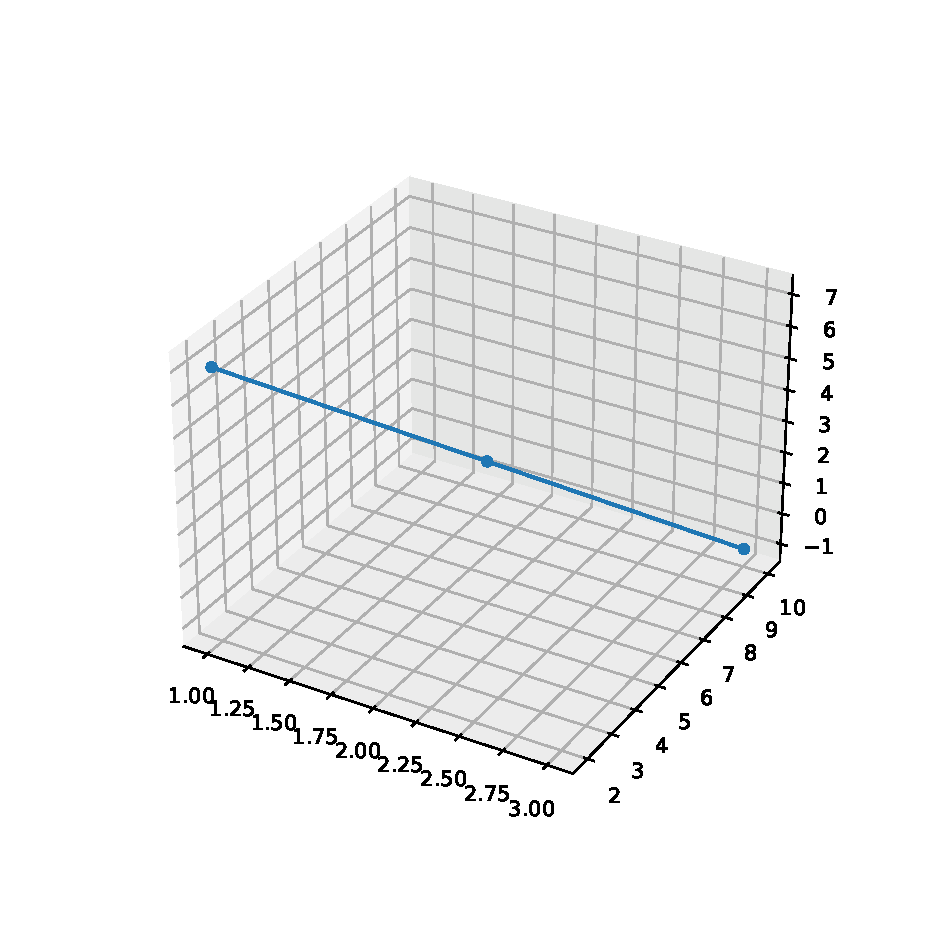
\includegraphics[width=\columnwidth]{figs/Plot.eps}
\end{figure}

\section{Generalizing Solution}

Let $\textbf{A}_{i} = \begin{pmatrix} x_{i,0} \\ x_{i,1} \\ \vdots \\ x_{i, n-1} \end{pmatrix}$ be an $n$ dimensional vector and it represents $i^{th}$ point where $i \in \{0,1,2,..,m-1\}$. The objective is to check whether these $m$-points are collinear or not.\\

For all the m-points to be collinear any three points among m-points $A_{i}$, $A_{j}$ and $A_{k}$ should be collinear i.e $\textbf{A}_{k}\textbf{A}_{i} = \lambda \times \textbf{A}_{j}\textbf{A}_{i}$.\\

\begin{align}
\textbf{A}_{k}\textbf{A}_{i} = \begin{pmatrix} x_{k,0} - x_{i,0} \\ x_{k,1} - x_{i,1} \\ \vdots \\ x_{k,n-1} - x_{i,n-1} \end{pmatrix} \\
\textbf{A}_{j}\textbf{A}_{i} = \begin{pmatrix} x_{j,0} - x_{i,0} \\ x_{j,1} - x_{i,1} \\ \vdots \\ x_{j,n-1} - x_{i,n-1} \end{pmatrix} \\
\begin{pmatrix} x_{k,0} - x_{i,0} \\ x_{k,1} - x_{i,1} \\ \vdots \\ x_{k,n-1} - x_{i,n-1} \end{pmatrix} = \lambda \begin{pmatrix} x_{j,0} - x_{i,0} \\ x_{j,1} - x_{i,1} \\ \vdots \\ x_{j,n-1} - x_{i,n-1} \end{pmatrix}
\end{align}

It can be rewritten as:
\begin{multline}
\frac{x_{k,0} - x_{i,0}}{x_{j,0} - x_{i,0}} = \frac{x_{k,1} - x_{i,1}}{x_{j,1} - x_{i,1}} = ... = \frac{x_{k,n-1} - x_{i,n-1}}{x_{j,n-1} - x_{i,n-1}} = \lambda
\end{multline}

So, if all m-points satisfy the above condition it can be concluded that all the points are collinear.

\end{document}
